\chapter{Results}
\label{chp:results}
% ---------------------------------------------------------------------------------------------------


\begin{itemize}
\itemsep0em
  \item emulator should never underestimate danger (what type of error is this? we want to avoid it absolutely)
  \item try to perform GP interpolation. If it does not work, explain why polynomial interpolation (no time)
  \item use emulator with uncertainty in the $I$ and $\theta_i$. Perform uncertainty quantification
\end{itemize}

% ===================================================================================================
\section{Classification emulator}
% ===================================================================================================

Results for the classification emulator
\begin{itemize}
  \item show classification with 3 different $Q_!$
  \item perform testing 
\end{itemize}

\begin{figure}[htpb]
  \centering
  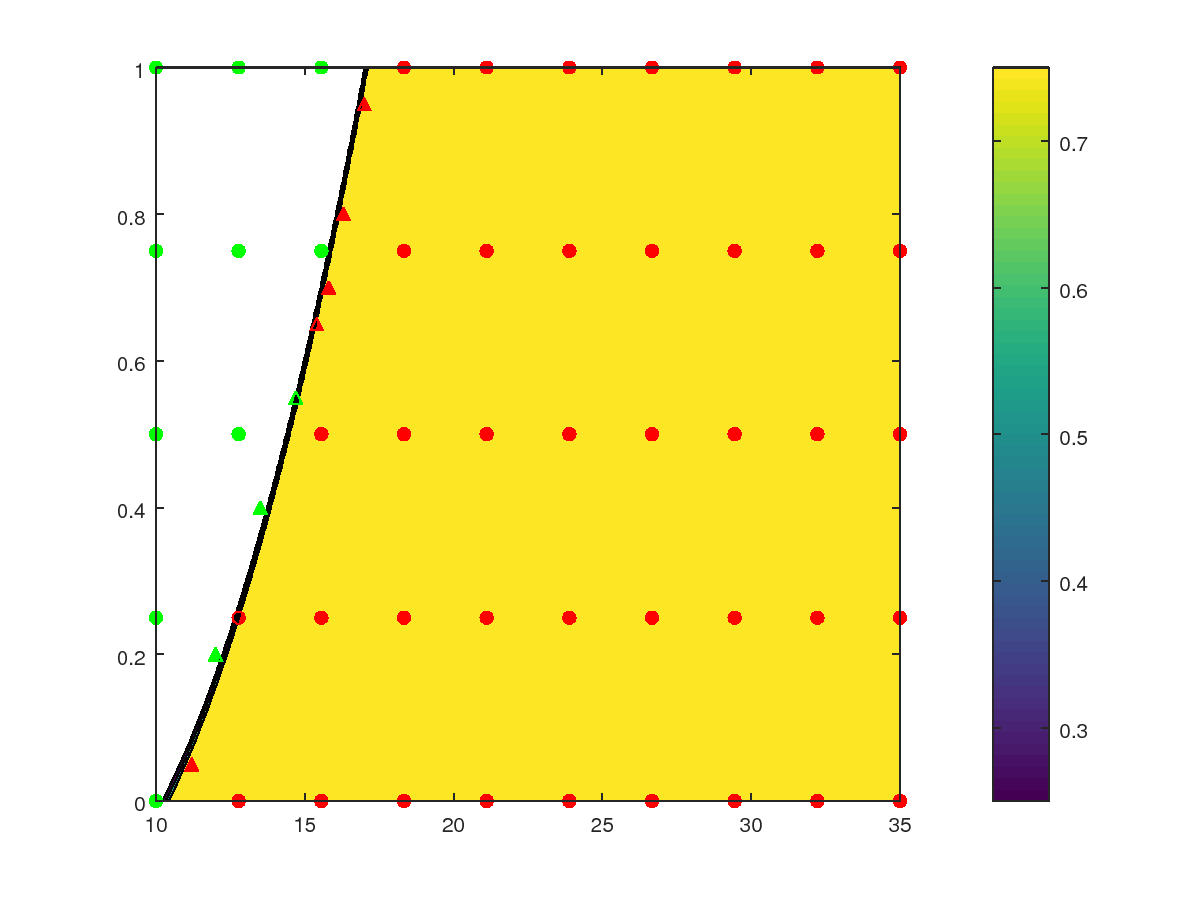
\includegraphics[width=0.75\textwidth]{Figures/classification.png}
  \caption{Binary classification emulator: events reaching $Q_!$ (red) and events not reaching $Q_!$ (green) for $Q_! = XX.X$.}
  \label{fig:classification_Q1}
\end{figure}

% ---------------------------------------------------------------------------------------------------
\subsection{Classification performance}
% ---------------------------------------------------------------------------------------------------


% ===================================================================================================
\section{An hydrological emulator: time to peak}
% ===================================================================================================

\begin{figure}[htpb]
  \centering
  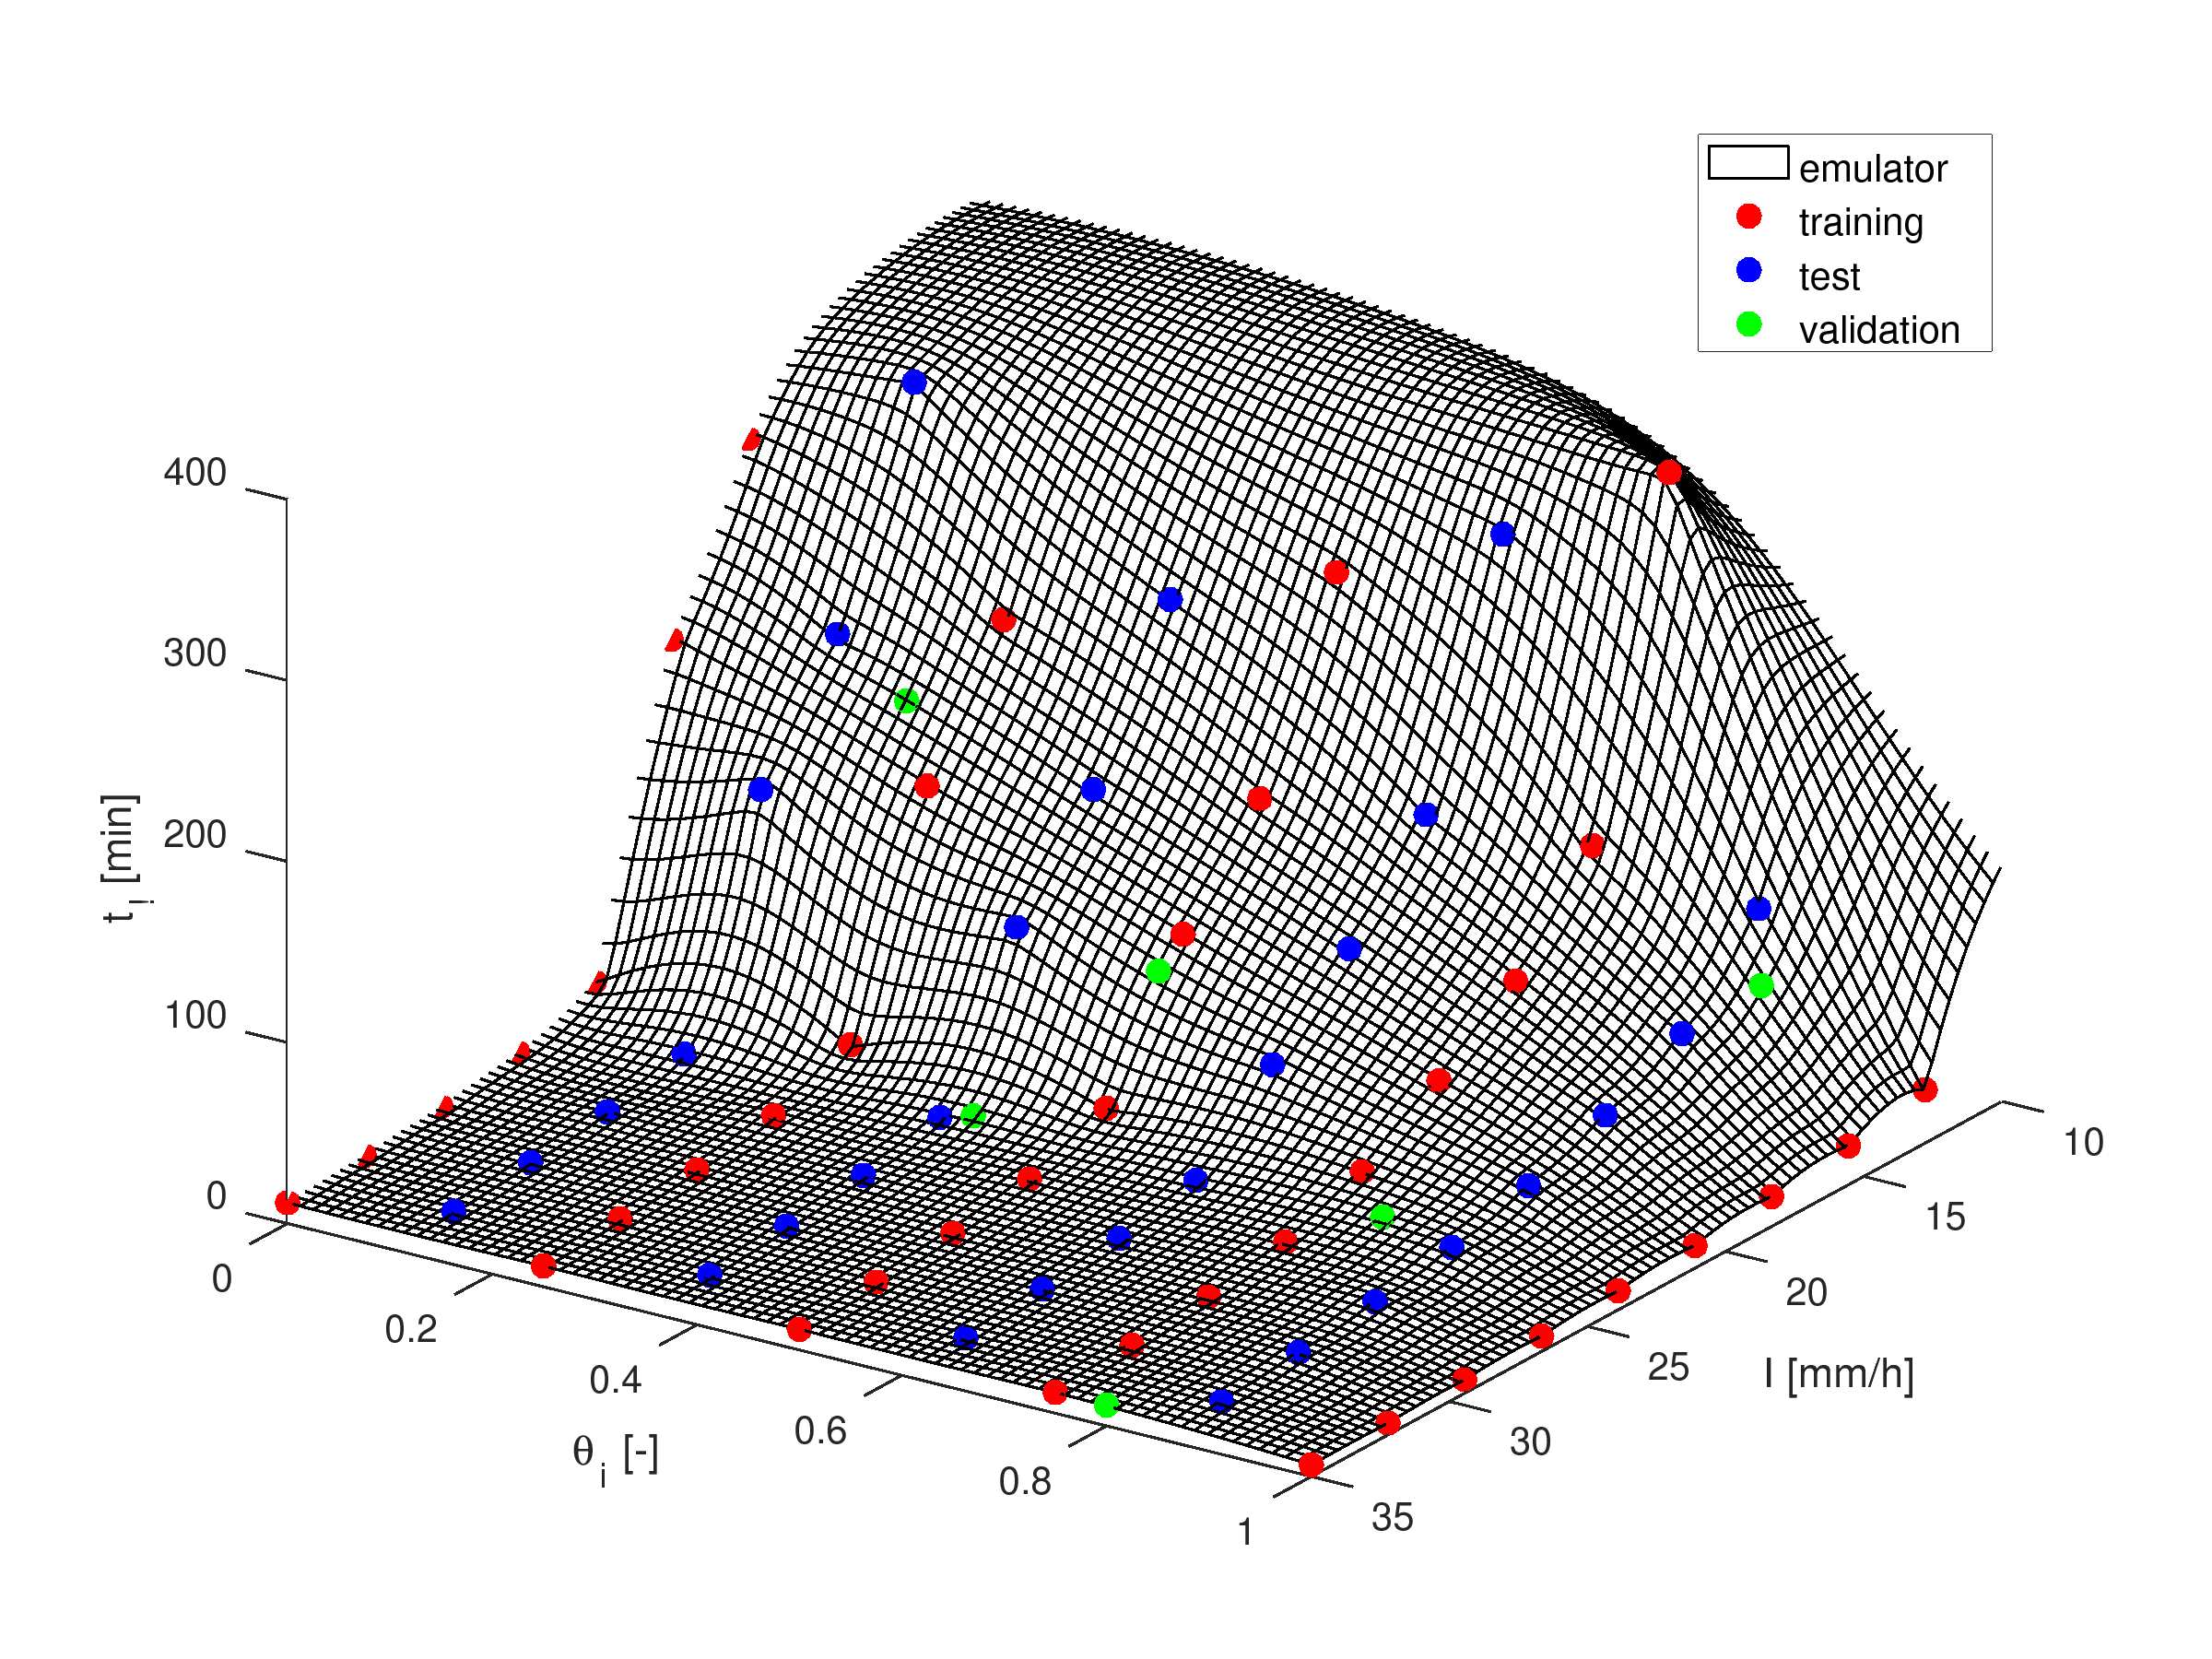
\includegraphics[width=0.7\textwidth]{Figures/emulator.png}
  \caption{Time-to-threshold emulator: training (red), test (blue) and validation (green) datasets and the emulator producing the intrapolation response.}
  \label{fig:}
\end{figure}

With this case study it was decided to address a complex hydrological problem by means of emulation.
The problem we want to solve is estimating the time needed for a channel conveying water from a catchment to 

% ---------------------------------------------------------------------------------------------------
\subsection{Material and methods}
% ---------------------------------------------------------------------------------------------------



\begin{table}[htpb]
  \centering
  \caption{Emulator performance on \emph{test} and \emph{validation} data}
  \label{table label}
  \begin{tabular}{lcc}
    \toprule
     & \textbf{MAE [\si{\minute}, \si{\percent}]} & \textbf{RMSE [\si{\minute}, \si{\percent}]} \\
    \midrule
    \textbf{test} & val & val \\
    \textbf{validation} & val & val \\
    \bottomrule
  \end{tabular}
\end{table}


% ---------------------------------------------------------------------------------------------------
\subsection{Parameters uncertainty propagation}
% ---------------------------------------------------------------------------------------------------





